\section{Presentation Logic Layer}

%What pages will be present in your project? briefly indicate how your web site will be organized

The website is divided into the following pages:
\begin{itemize}
    \item \textbf{Homepage}: contains the showcase of the featured products and the available products.
    \item \textbf{Product page}: allows the customer to inspect all the information about a given product. To buy the product the customer has to be logged in.
    \item \textbf{Login page}: allows both customers and employees to login. 
    \item \textbf{Order list and Order details page}: allow each customer to look at their order history, to open a ticket, cancel the order or get the invoice.
    \item \textbf{Tickets page}: allows each customer to look at their ticket history. There exists an employee version of the page to manage each ticket.
    \item \textbf{Product management pages}: both simple employees and administrators are able to look at all the products and create/edit/delete them. Through a second page (Discount management) it is also possible to add some discounts to the products.
    \item \textbf{Orders management page}: both simple employees and administrators are able to look at all the orders and edit/cancel them. It's also possible to look at the existing invoices for each product.
    \item \textbf{User edit page}: allows both customers and employees to modify their personal data. 
    \item \textbf{Administration page}: allows the administrators to edit the name, surname, role of all the users and even delete their account.
\end{itemize}

\subsection{Homepage}
    \begin{figure}[H]
        \centering
        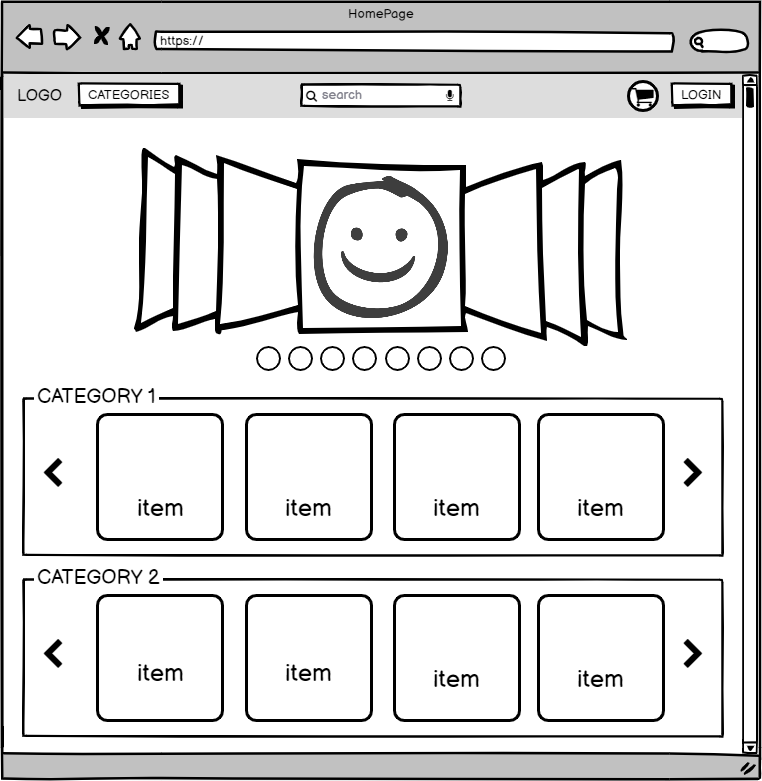
\includegraphics[width=\textwidth,height=0.7\textheight,keepaspectratio]{mockups/homepageMockup.png}
            \caption{Homepage: main page of the web application}
            \label{fig:Homepage}
    \end{figure}

The homepage contains the main information regarding the various products available.
The products are divided into subsets according to their category. This subdivision will be done by using a scrollable list. Moreover, the homepage contains a search bar that allows a user to search a product by its name.
The homepage contains a status bar that allows the user to register, log in or log out once logged in.
Finally, this status bar allows customers to show the history of the products purchased.

\subsection{Product page}
    \begin{figure}[H]
        \centering
        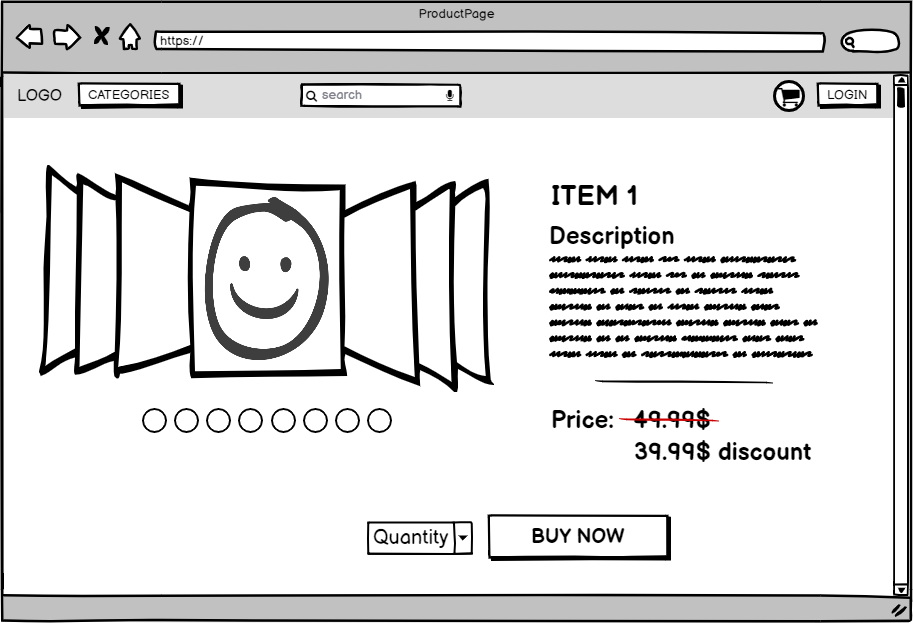
\includegraphics[width=\textwidth,height=0.7\textheight,keepaspectratio]{mockups/productPageMockup.png}
            \caption{Product Page: page regarding the details of a product}
            \label{fig:ProductPage}
    \end{figure}

The product page shows in detail the information regarding a specific product.
This page shows all the pictures available for the product, the description and its price.
In addition, it also shows any discount applied to the product at the moment.
If the customer is logged in, it will be possible for him to purchase the product within the maximum quantity available. It is possible to enter these particular pages by clicking on a product from the homepage, from the specific category page or by searching it by name using the search bar.

\subsection{OrderList and OrderDetails}
    \begin{figure}[H]
        \centering
        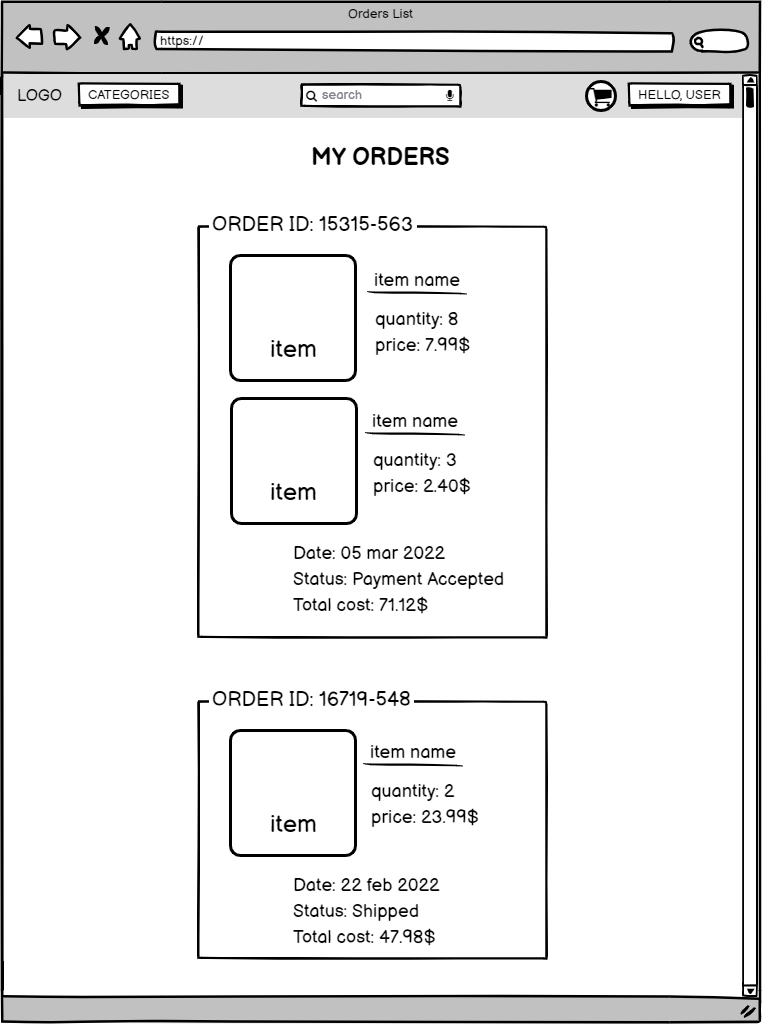
\includegraphics[width=\textwidth,height=0.7\textheight,keepaspectratio]{mockups/ordersPageMockup.png}
            \caption{Order list page: page regarding all the orders of the logged customer}
            \label{fig:OrderPage}
    \end{figure}

This page shows in detail all the orders placed by the customer which is currently logged in. It shows the history of all orders placed since the user's registration till now. For each order, it shows the date, the total price and the status.
Furthermore, for each order, there is a list of all the products purchased, their quantity and their unit price at the time of purchase.

\subsection{Ticket list management}
    \begin{figure}[H]
        \centering
        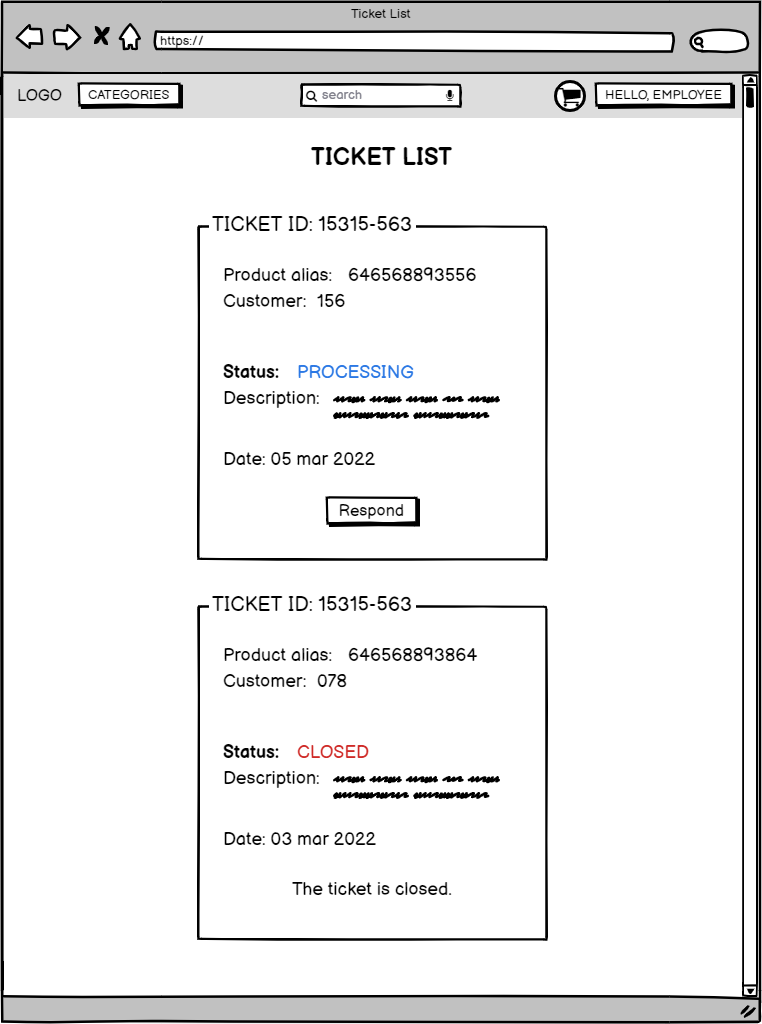
\includegraphics[width=\textwidth,height=0.7\textheight,keepaspectratio]{mockups/ticketPageMockup.png}
            \caption{Ticket list management page: page regarding all the tickets opened}
            \label{fig:TicketPage}
    \end{figure}
The ticket list page can be accessed by both customers and employees. In the customer version, the page shows the list of the ticket opened by the current user. Each ticket displays its ID, its status and the product involved. In the employee version, each ticket shows also the ID of the customer. Furthermore, this page allows the employee to respond to the ticket and update its status.


\subsection{UserEdit page}
    \begin{figure}[H]
        \centering
        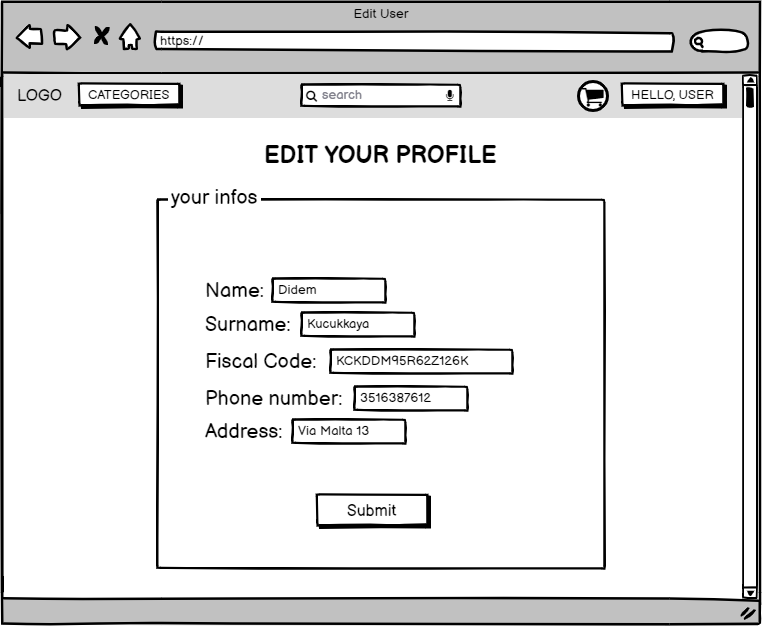
\includegraphics[width=\textwidth,height=0.7\textheight,keepaspectratio]{mockups/userEditPageMockup.png}
            \caption{User edit page: page that allows the current user to edit their informations}
            \label{fig:UserEdit}
    \end{figure}

The user edit page allows the customer type user to change its personal data. The page consist of text boxes with default values corresponding to the values previously entered by the user. The page allows you to change data such as telephone number, name, surname but not unique / primary key, because this particular data is used for the login.
Obviously, this page will be available only if the user is logged in.

    
\subsection{Admin: product management} 
    \begin{figure}[H]
        \centering
        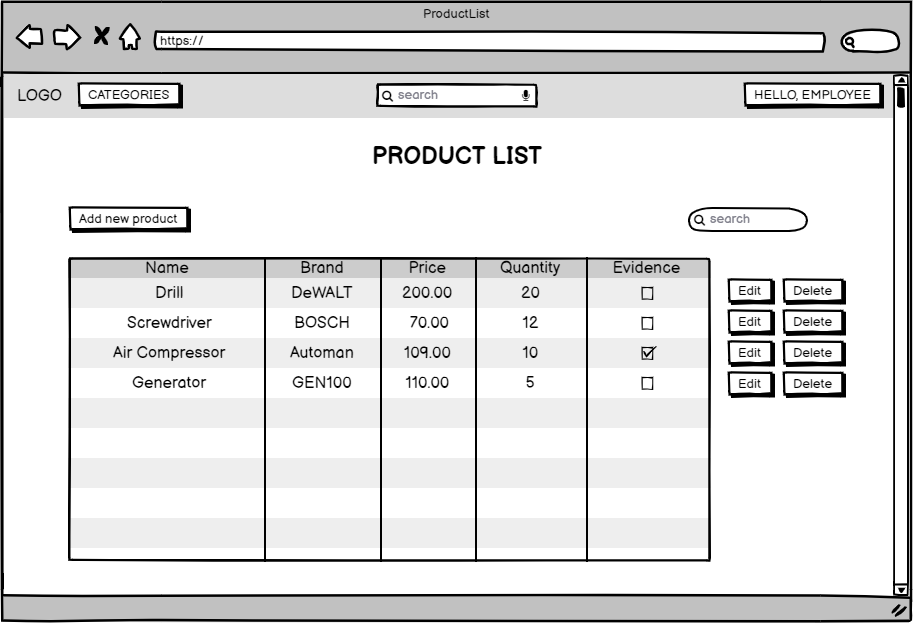
\includegraphics[width=\textwidth,height=0.7\textheight,keepaspectratio]{mockups/productListPageMockup.png}
            \caption{Product management page: page that shows all the products of the shop}
            \label{fig:ProductManagement}
    \end{figure}
Only the employees have access to the product management pages (as well as administrators). 
The page, which refers to the management of products, allows the employees to view a table, which lists all the products of the e-shop, with their information, such as name, the brand, the selling price and the quantity. 
In addition, the page gives the possibility to edit the products. However, let's reiterate that products can't be deleted in any case: the only way to "logically delete" a product is by setting its quantity to zero. In this manner, products with a quantity equal to zero are unseen, therefore unavailable for the purchase. 
Finally there's an "add a new product" button for the creation of a new product to the list (see fig.\ref{fig:ProductManagementAdd}). Since every product belongs to a specific category, it is also possible to create a new category when adding a new product, or just use an existing one.

Thanks to this page, the owner of the e-shop will be able to upgrade his selling activity and offer more products in his catalogue. 
    
    \begin{figure}[H]
        \centering
        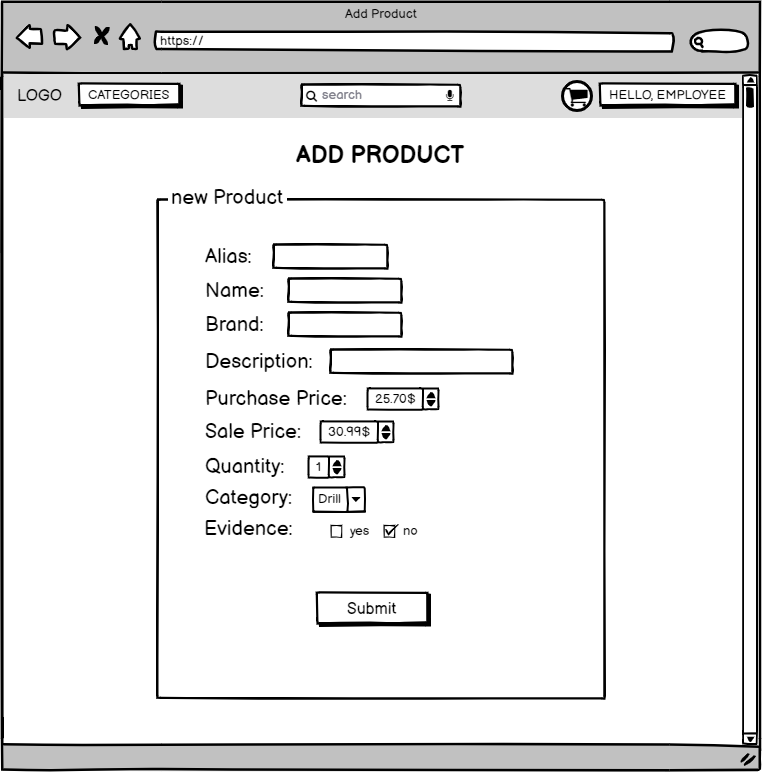
\includegraphics[width=\textwidth,height=0.7\textheight,keepaspectratio]{mockups/addProductPageMockup.png}
            \caption{Add product page: page that allows to add a new product}
            \label{fig:ProductManagementAdd}
    \end{figure}



\subsection{Admin: user management}
    \begin{figure}[H]
        \centering
        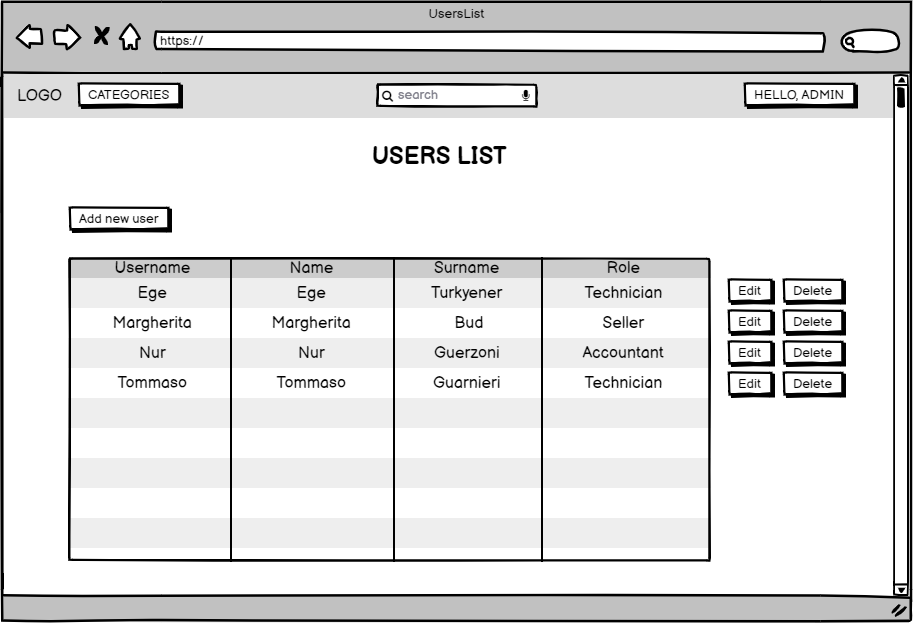
\includegraphics[width=\textwidth,height=0.7\textheight,keepaspectratio]{mockups/usersListPageMockup.png}
            \caption{User management page: page that shows all users}
            \label{fig:UserManagement}
    \end{figure}
    The user management page can be reached only by administrators. The page displays the username, name, surname and role of any employee registered in the website. It is also possible to edit, add, or delete a user.
    There exist two types of pages about "user management": one only for the employees and another for all the customers registered to the website.

